\documentclass[12pt,a4paper]{report}

%
% PACKAGES AND STYLES
%

% 
% Language and encoding
%
%\usepackage{mathtext}
%\usepackage[T2A]{fontenc}
\usepackage[utf8]{inputenc}
\usepackage[english,russian]{babel}
\usepackage{mmap}

%
% Colors
%
\usepackage[usenames]{color}
\usepackage{color}
\usepackage{colortbl}

%
% Symbols
%
\usepackage{amssymb}
\usepackage{MnSymbol}

%
% Units
%
%\usepackage[binary-units=true]{siunitx}
\newcommand{\km}{\mathrm{~\text{км}}}
\newcommand{\m}{\mathrm{~\text{м}}}
\newcommand{\s}{\mathrm{~\text{с}}}
\newcommand{\mps}{\m \s ^{-1}}
\newcommand{\pers}{\s ^{-1}}
\newcommand{\K}{\mathrm{~\text{К}}}
\newcommand{\Kpkm}{\K\km ^{-1}}
\newcommand{\hpa}{\mathrm{~\text{гПа}}}
\newcommand{\J}{\mathrm{~\text{Дж}}}
\newcommand{\Jpm}{\J \m ^{-3}}

%
% Paper size and margins
%
\usepackage{vmargin}
\setmarginsrb{2.5cm}{1cm}{2.5cm}{2cm}{0cm}{0cm}{0cm}{1.5cm}

%
% Page style
%
\usepackage{fancyhdr}
\setlength{\headheight}{16pt}
\newcommand{\changefont}{%
    \fontsize{9}{11}\selectfont
}
\fancyhf{}
\fancyhead[RO]{\changefont \slshape \rightmark} %section
\fancyhead[LO]{\changefont \slshape \leftmark} %chapter
\fancyfoot[C]{\changefont \thepage} %footer
\setlength{\headsep}{0.2in}
\pagestyle{fancy}

%
% Indenting
%
\usepackage{indentfirst}
\setlength{\parindent}{1cm}
\setlength{\parskip}{0.5cm}

%
% References
%
\usepackage{natbib}

%
% Hyperlinks
%
\usepackage[linktocpage=true,plainpages=false,pdfpagelabels=false]{hyperref}
\definecolor{linkcolor}{rgb}{0.1,0,0.9}
\definecolor{citecolor}{rgb}{0,0,0.9}
\definecolor{urlcolor}{rgb}{0,0,1}
\hypersetup{
    colorlinks, linkcolor={linkcolor},
    citecolor={citecolor}, urlcolor={urlcolor}
}

\bibliographystyle{plainnat}
% Bibliography: set article volume number in bold font
%\DeclareFieldFormat
%  [article]
%  {volume}{\textbf{#1}}
%\renewcommand\nameyeardelim{, }

%\usepackage{showkeys} % show labels

\newcommand{\figref}[1]{\mbox{Figure~\ref{#1}}}
\newcommand{\tabref}[1]{\mbox{Table~\ref{#1}}}
\newcommand{\secref}[1]{\mbox{Section~\ref{#1}}}
\newcommand{\chpref}[1]{\mbox{Chapter~\ref{#1}}}
\newcommand{\appref}[1]{\mbox{Appendix~\ref{#1}}}
\newcommand{\eqnref}[1]{\mbox{Eq.~(\ref{#1})}}
\newcommand{\listref}[1]{\mbox{Listing~(\ref{#1})}}

%
% Lists
%
\usepackage[shortlabels]{enumitem}

\newenvironment{sqlist}[1][\enskip$\filledsquare$]
        {\begin{itemize}[#1]}
        {\end{itemize}}

% New math commands
% differential d, from http://tex.stackexchange.com/a/60546/586
\newcommand*\diff{\mathop{}\!\mathrm{d}}
\newcommand\mean[1]{\overline{#1}}
\newcommand{\PDt}[2]{\partial #1/\partial #2}

%
% Tables
%
\usepackage{booktabs}
%\usepackage{tabularx}
\usepackage{tabu}
\usepackage{longtable}

%
% Figures
%
\usepackage{wrapfig}
\usepackage[font=small,textfont=it,labelfont=bf]{caption}
%\captionsetup[figure]{labelfont=bf}
\usepackage{tikz}
\usepackage{pgfplots}
\usetikzlibrary{calc}

%
% Equations
%
\usepackage{cool}


\begin{document}
\setcounter{chapter}{3}
\chapter{Результаты}
Данный раздел посвящен обзору результатов численного моделирования, постановка которых описана выше. Раздел построен следующим образом: сначала рассматривается контрольный эксперимент, а именно структура, динамика и энергетика вихря. Затем аналогичным образом описывается эксперимент со включенной параметризацией микрофизики, и оценивается чувствительность вихря к начальному содержанию влаги в атмосфере.

\begin{wrapfigure}{l}{0.5\textwidth}
\begin{center}
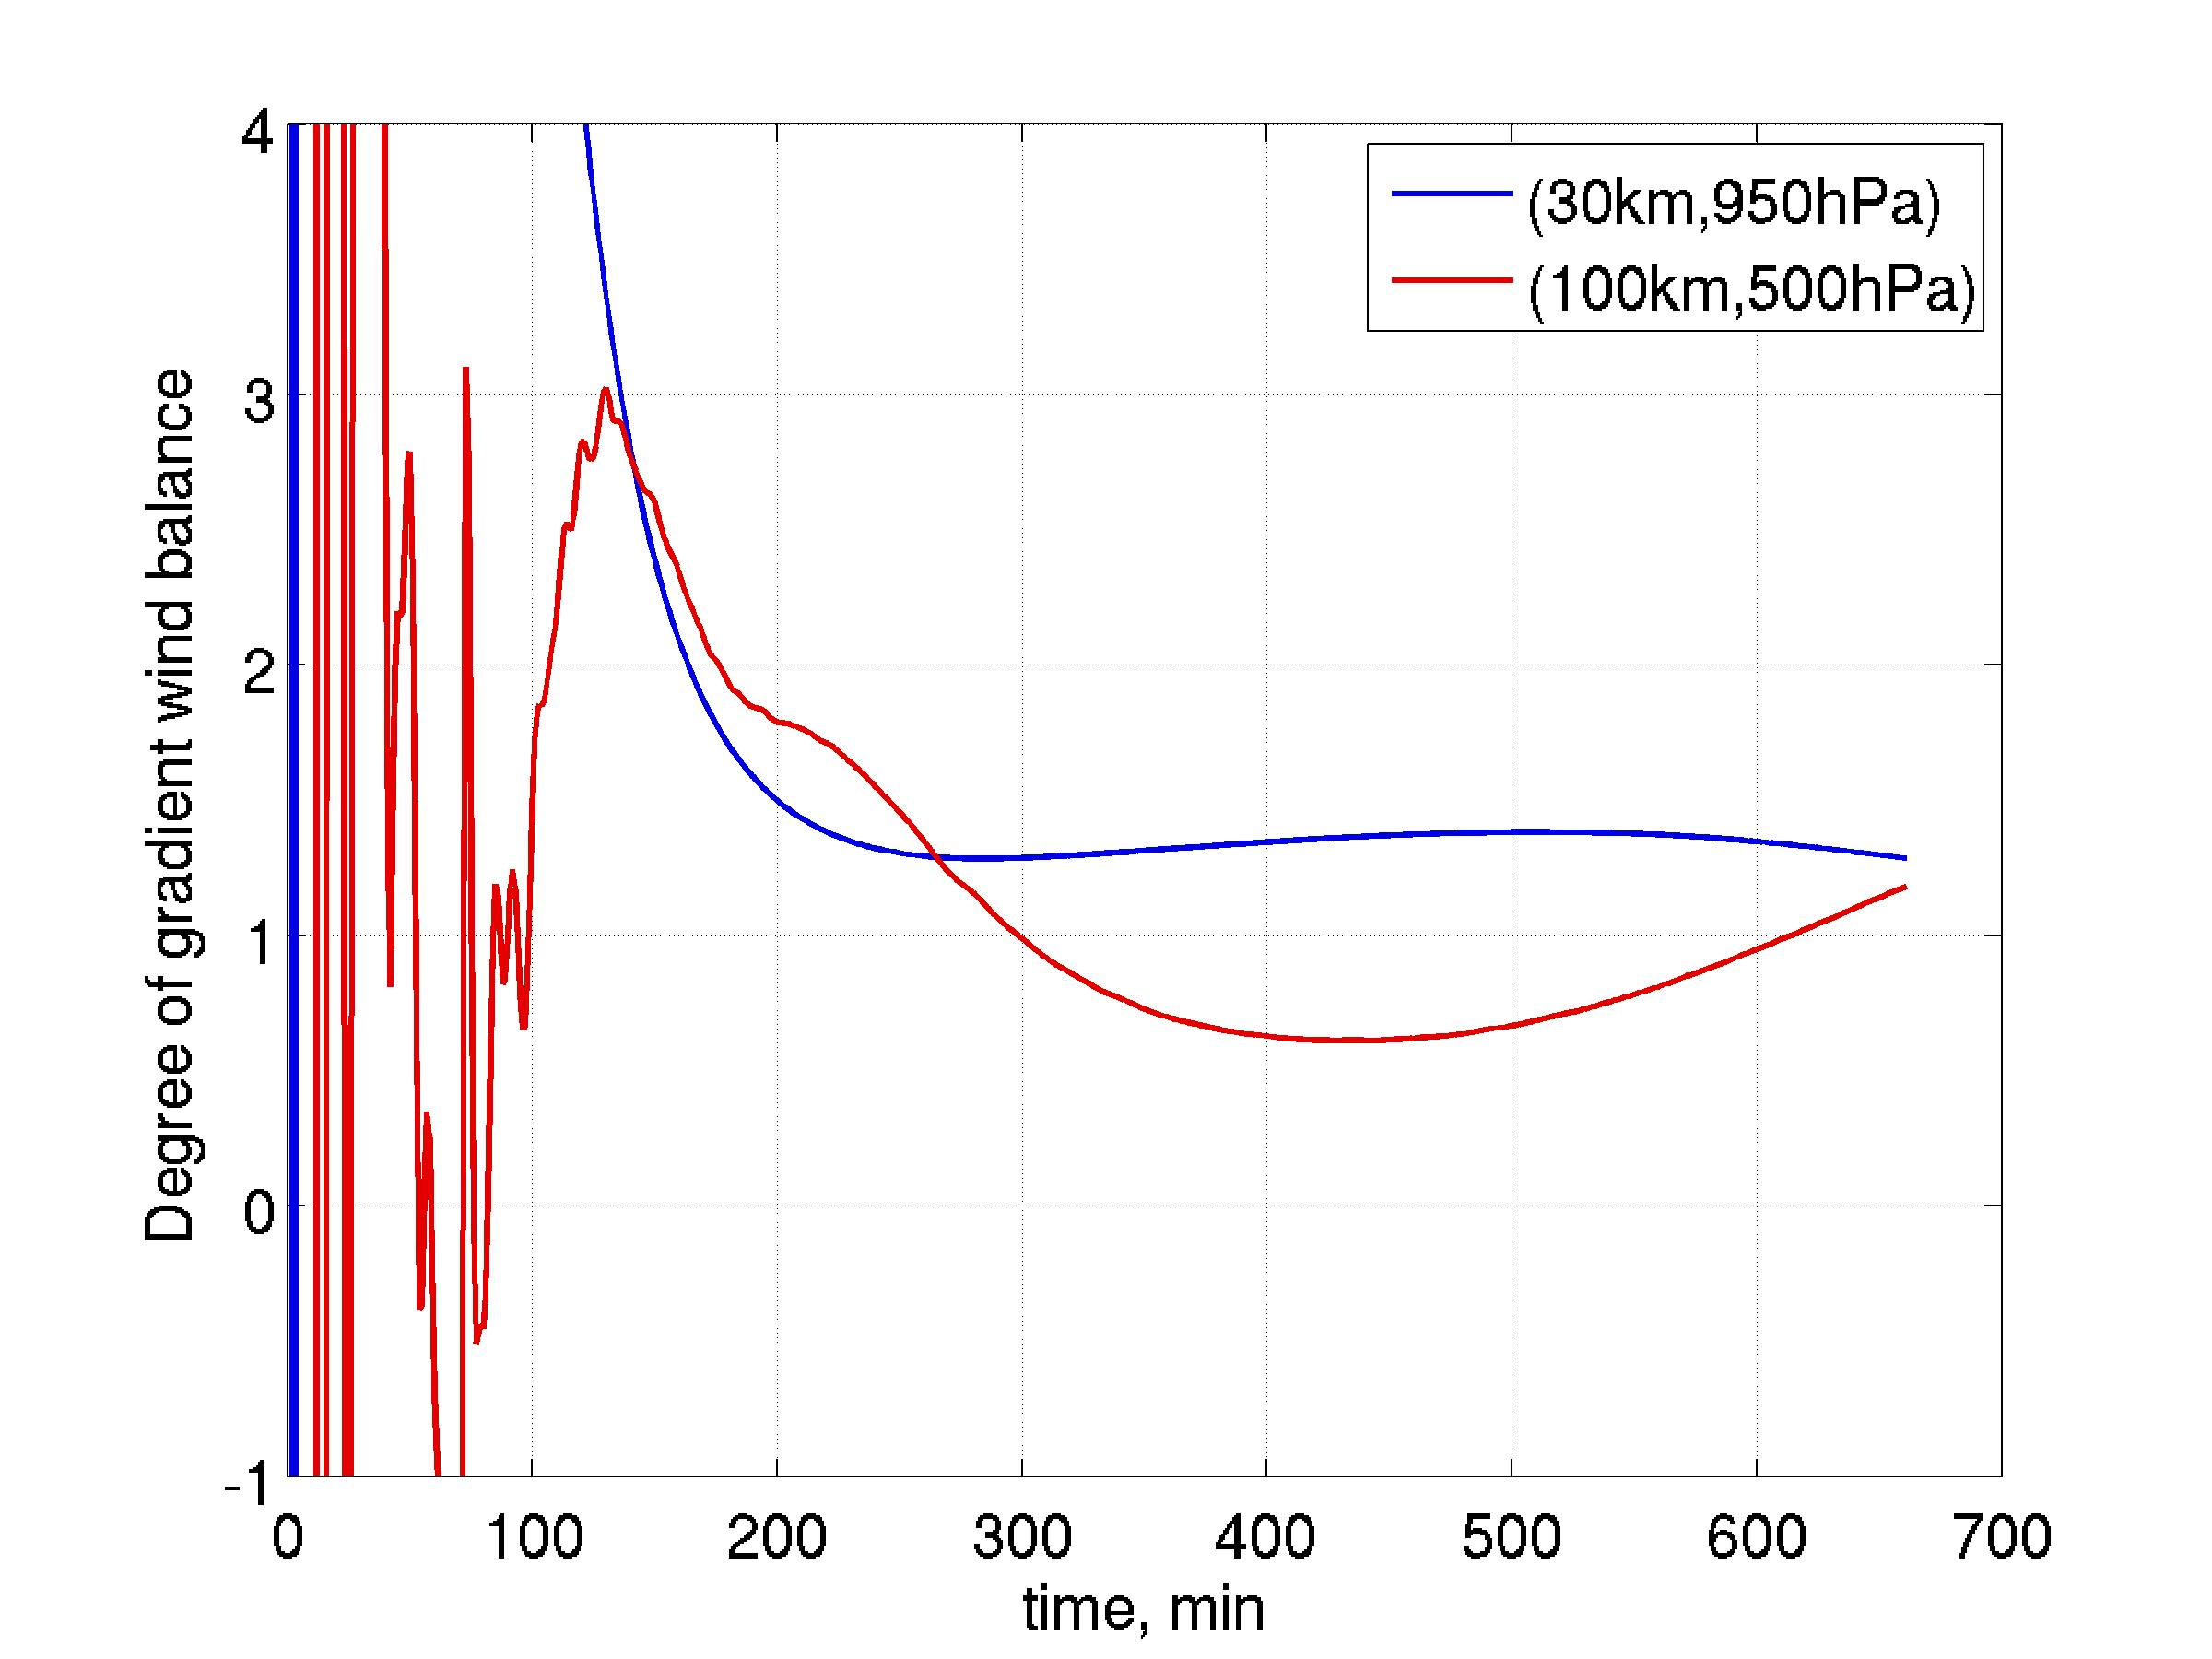
\includegraphics[scale=0.1]{{./chapters/figures_results/ctrl_grwindbal2p}.jpg}
\end{center}
\caption{Величина градиентного баланса $\pderiv{\phi'}{r}/\left(v^2_t/r+fv_t\right)$ как функция времени с момента инициализации возмущения: при $r=30\km, p=950\hpa$ (синяя кривая) и при $r=100\km, p=500\hpa$ (красная кривая). Градиентный баланс достигается, когда кривые приближаются к $1$.}
\label{fig:grwindbal}
\end{wrapfigure}
Влияние остальных факторов на динамику мезоциклона рассматривается с точки зрения таких интегральных характеристик, как кинетическая энергия, максимальная завихренность, минимальное приземное давление. Для интерпретации различий в результатах оценочных экспериментов привлекается анализ пространственной структуры метеополей.

Полярный мезоциклон в каждом эксперименте развивался с разной скоростью, и продолжительность экспериментов составляет 1-3 сут. Трехмерные поля в каждый момент времени интерполируются на регулярную сетку с горизонтальным разрешением, соответствующим разрешению модели. В экспериментах без фонового потока горизонтальные разрезы сфокусированы на район развития вихря (обычно $200\times 200\km$ в центре области). По вертикали данные интерполируются на регулярную сетку с шагом $500\m$ для удобства последующего постпроцессинга. В некоторых экспериментах также используется интерполяция на изобарические поверхности от $1000$ до $250\hpa$ с шагом $50\hpa$.

\section{Контрольный эксперимент}
\subsection{Начальная стадия развития вихря}
Начнем с рассмотрения момента инициализации температурной аномалии. Ее форма и начальная амплитуда видна на рис. \ref{}. 

Появление источника тепла в атмосфере, находящейся в равновесии, ставит проблему реакции атмосферы и достижения нового баланса через механизм приспособления. Этот вопрос впервые был развит Лэмбом \citep{RT2003}, который изучал особенности волн, излучаемых в процессе гидростатического приспособления. Позднее эта проблема была обобщена как ответ устойчиво стратифицированной атмосферы на вертикально ограниченный, но горизонтально однородный источник тепла. Один из интересных результатов, полученных в работе \citep{Bannon1995}, заключаются в том, что если источник тепла горизонтально однороден, то слои воздуха ниже источника не смещаются относительно начального положения. Слои же воздуха выше источника одинаково подняты вверх. Источник нагрева в нижней тропосфере влияет на распределение давления во всей толще атмосферы выше него. Для оценки высоты, на которую распространяется влияние нагрева снизу в работе \citep{Bannon1995} было введено понятие вертикальный масштаб возмущения применительно к изотермической атмосфере. При этом в атмосфере с реалистичной структурой этот масштаб несильно отличается от такового для изотермической атмосферы. Так как распределение давления больше всего меняется на верхней границе нагретого слоя, и ответ поля давления на источник тепла убывает с высотой экспоненциально, в случае нагрева нижних слоев тропосферы эффект будет проявляться главным образом в тропосфере.

Более интересно для реальной атмосферы рассмотреть проблему Лэмба для случая неоднородного источника тепла. Например, если взять источник тепла определенного радиуса, то он будет излучать не только вертикально распространяющийся горизонтальный волновой фронт, но и сферический волновой фронт, распространяющийся от внешнего радиуса аномалии горизонтально и вертикально. 

Подобный процесс наблюдается в начале каждого эксперимента данной работы. Ввиду того, что нагрев в районе аномалии происходит не мгновенно, а в течение конечного отрезка времени, как и бывает в реальной атмосфере,  фронт излучаемых волн прослеживается слабее. Тем не менее, результат качественно совпадает идеализированными экспериментами \citep{RT2003}. Вертикальный барический градиент находится почти в гидростатическом балансе с силой плавучести, а горизонтальный создает циклоническую циркуляцию. Такая циркуляция возникает в устойчиво стратифицированной атмосфере, и источник энергии в виде конвективной доступной потенциальной энергии (CAPE) не является необходимым. При остановке подачи тепла не вращающаяся атмосфера постепенно придет к состоянию покоя. Однако это не так, если атмосфера испытывает вращение, что подтверждается в наших экспериментах \ref{sec:res:nohle}.

Начальная куполообразная аномалия приводит к возникновению в нижних слоях атмосферы горизонтального градиента давления, который создает конвергенцию массы в центре области (рис. \ref{}). В результате под влиянием силы Кориолиса возникают инерционно-гравитационные волны, в то время как возникновение звуковых волн невозможно ввиду разрешения сетки модели (\citep{MillerWhite1984,MirandaPhD}). Путем излучения инерционно-гравитационных волн происходит приспособление атмосферы к геострофическому балансу (рис. \ref{fig:grwindbal}).


Вертикальный разрез вертикальной скорости \ref{} дает представление о распространении гравитационных волн в ответ на температурное возмущение. Рисунок схож с результатами линейной теории \citep{Lin2007}, однако более правдоподобен из-за нелинейности процессов и интерференции волн в реальной атмосфере. При задании неоднородного фонового профиля стратификации области подъема и нисхождения воздуха, очевидно, будут иметь несимметричную форму.

Несмотря на четко различимые в начале моделирования волны, их влияние мало: аномалия потенциального вихря, определяющая циркуляцию в атмосфере, остается на месте, где она была изначально помещена. Другими словами, возмущение потенциального вихря не переносится вместе с инерционно-гравитационными волнами \citep{RT2003}. Влияние волн, созданных начальным дисбалансом в атмосфере пренебрежимо мало по сравнению с “равновесной” частью движения, которое связано через принцип обратимости с распределением потенциального вихря.

Равновесная часть движения формируется сразу после инициализации температурной аномалии. Подтверждением того, что наибольший вклад в развитие циркуляции имеет конвергенция массы, служит анализ уравнения завихренности в изобарической системе координат \citep{Bluestein1992I} для $f$-плоскости:
\begin{equation}
\pderiv{\zeta}{t}=-v\dot{}...,
\end{equation}
где $\zeta$ – вертикальная компонента вектора вихря скорости (завихренность).
Рассмотрим состояние эксперимента в 3 час модельного времени – в момент, когда аномалия только что была инициализирована. На рис. \ref{} представлены пространственное распределение компонент, входящих в правую часть ур. \ref{}. Данные осреднены по вертикали в слое от 0 до 1000 м, в котором в течение всего времени наблюдаются наибольшие значения градиентов скорости.

Нетрудно заметить, что содержащее горизонтальную дивергенцию слагаемое (слагаемое растяжения) имеет наибольшие значения, причем его экстремум совпадает с экстремумом тенденции завихренности и они близки по значению. Недостающую часть тенденции вихря составляет вертикальная адвекция. Величина завихренности уже достаточно велика в данный момент (приблизительно в 2 раза меньше, чем значение параметра Кориолиса), а скорость ее роста говорит о том, что меньше, чем через час значения удвоятся. Бароклинное слагаемое (\ref{}) – произведение градиентов давления и плотности – имеет значения на 3-4 порядка меньшие остальных членов, и это соотношение сохраняется в течение всего эксперимента. Поэтому далее бароклинное слагаемое рассматриваться не будет.





\begin{thebibliography}{12}
 \bibitem{ER89}
Emanuel KA, Rotunno R. 1989. Polar lows as Arctic hurricanes. \textit{Tellus} \textbf{41A:} 1-17.
\end{thebibliography}

\end{document}